%! Author = user
%! Date = 3/9/2024

% Preamble
\documentclass{article}
\usepackage[utf8]{inputenc}
\usepackage{amsmath, amssymb, amsthm}
\usepackage{tikz}
\usepackage{pgfplots}
\usepackage{subfigure}
\usepackage{listings}
\usepackage[fontsize=13pt]{fontsize}
\usepackage[a4paper,
            bindingoffset=.2in,
            left=.7in,
            right=.7in,
            top=1in,
            bottom=1in,
            footskip=.25in]{geometry}

\definecolor{dkgreen}{rgb}{0,0.6,0}
\definecolor{gray}{rgb}{0.5,0.5,0.5}
\definecolor{mauve}{rgb}{0.58,0,0.82}

\lstset{frame=tb,
  language=Java,
  aboveskip=3mm,
  belowskip=3mm,
  showstringspaces=false,
  columns=flexible,
  basicstyle={\small\ttfamily},
  numbers=none,
  numberstyle=\tiny\color{gray},
  keywordstyle=\color{blue},
  commentstyle=\color{dkgreen},
  stringstyle=\color{mauve},
  breaklines=true,
  breakatwhitespace=true,
  tabsize=3
}

\title{LaTex for Students}
\author{Jun Ho Lee}
\date{March 2024}

% Document
\begin{document}

\newpage
\section{Week3}

Shallow Neural Network.

\subsection{Neural Network Overview}

What is a Neural Network?\\

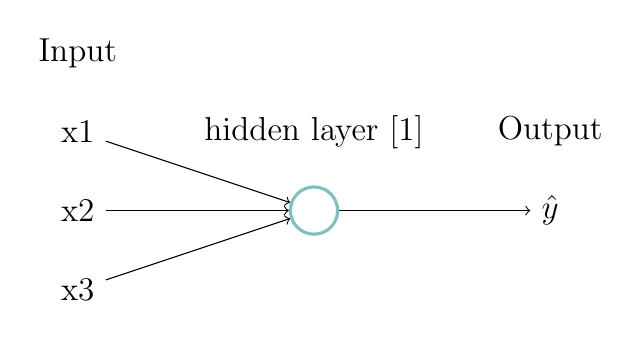
\begin{tikzpicture}
    % Input Layer
    \foreach \name/\i in {x1/1,x2/2,x3/3} {
        \node (Input-\i) at (0,-\i) {\name};
        \ifnum \i=1
            \node[above of=Input-\i] {Input};
        \fi
    }
    % Hidden Layer
    \foreach \i in {1} {
        \node[circle, minimum size = 6mm, draw=teal!50, line width=.4mm] (Hidden1-\i) at (3,-2) {};
        \ifnum \i=1
        \node[above of=Hidden1-\i] {hidden layer $[1]$};
        \fi
    }
    % Output Layer
    \foreach \name/\i in {$\hat{y}$/1} {
        \node (Output-\i) at (6,-2) {\name};
        \ifnum \i=1
        \node[above of=Output-\i] {Output};
        \fi
    }
    % Arrows
    \foreach \i in {1,2,3} {
        \foreach \j in {1} {
           \draw[->] (Input-\i) -- (Hidden1-\j);
        }
    }
    \foreach \i in {1} {
        \foreach \j in {1} {
            \draw[->] (Hidden1-\i) -- (Output-\j);
        }
    }
\end{tikzpicture}


$\fbox{$x, w, b$} \rightarrow \fbox{$z=w^T x + b$} \rightarrow \fbox{$a=\sigma(z)$} $\\\\


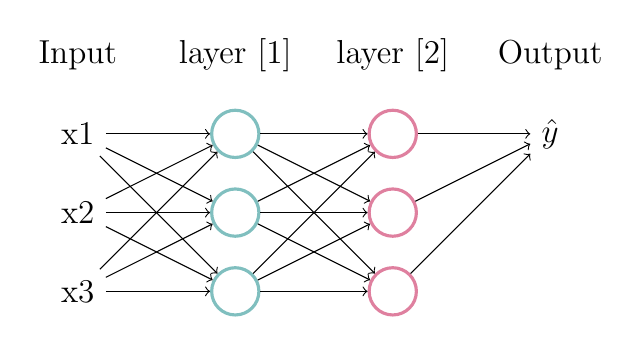
\begin{tikzpicture}
    % Input Layer
    \foreach \name/\i in {x1/1,x2/2,x3/3} {
        \node (Input-\i) at (0,-\i) {\name};
        \ifnum \i=1
            \node[above of=Input-\i] {Input};
        \fi
    }
    % Hidden Layer
    \foreach \i in {1,2,3} {
        \node[circle, minimum size = 6mm, draw=teal!50, line width=.4mm] (Hidden1-\i) at (2,-\i) {};
        \ifnum \i=1
        \node[above of=Hidden1-\i] {layer $[1]$};
        \fi
    }
    \foreach \i in {1,2,3} {
        \node[circle, minimum size = 6mm, draw=purple!50, line width=.4mm] (Hidden2-\i) at (4,-\i) {};
        \ifnum \i=1
        \node[above of=Hidden2-\i] {layer $[2]$};
        \fi
    }
    % Output Layer
    \foreach \name/\i in {$\hat{y}$/1} {
        \node (Output-\i) at (6,-\i) {\name};
        \ifnum \i=1
        \node[above of=Output-\i] {Output};
        \fi
    }
    % Arrows
    \foreach \i in {1,2,3} {
        \foreach \j in {1,2,3} {
           \draw[->] (Input-\i) -- (Hidden1-\j);
        }
    }
    \foreach \i in {1,2,3} {
        \foreach \j in {1,2,3} {
           \draw[->] (Hidden1-\i) -- (Hidden2-\j);
        }
    }
    \foreach \i in {1,2,3} {
        \foreach \j in {1} {
            \draw[->] (Hidden2-\i) -- (Output-\j);
        }
    }
\end{tikzpicture}


$\fbox{$x, W^{[1]}, b^{[1]}$} \rightarrow \fbox{$z^{[1]} = W^{[1]} x + b^{[1]}$} \rightarrow \fbox{$a^{[1]} = \sigma(z^{[1]})$} \\
\rightarrow \fbox{$z^{[2]} = W^{[2]} x + b^{[2]}$} \rightarrow \fbox{$a^{[2]} = \sigma(z^{[2]})$} \rightarrow \fbox{$\mathcal{L}(a^{[2]},y)$} $\\


\newpage
\subsection{Neural Network Representations}

Values of the input features (activation): $ X = a^{[0]}$\\

The following is the 2-Layer Neural Network:\\

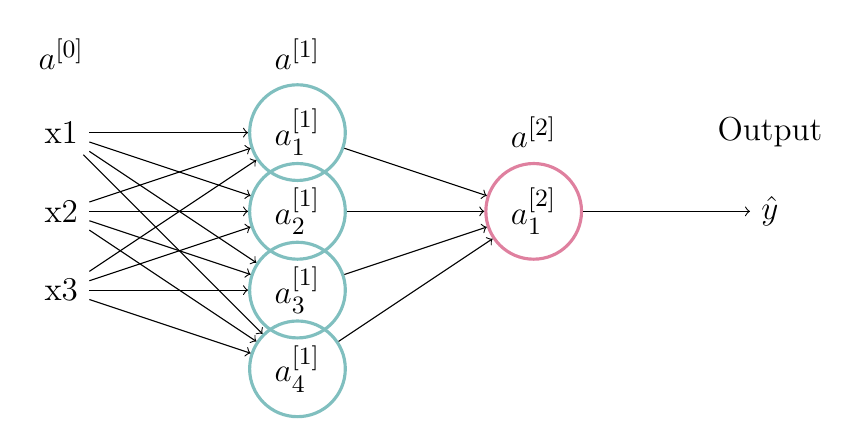
\begin{tikzpicture}
    % Input Layer
    \foreach \name/\i in {x1/1,x2/2,x3/3} {
        \node (Input-\i) at (0,-\i) {\name};
        \ifnum \i=1
            \node[above of=Input-\i] {$a^{[0]}$};
        \fi
    }
    % Hidden Layer
    \foreach \i in {1,2,3,4} {
        \node[circle, minimum size = 6mm, draw=teal!50, line width=.4mm] (Hidden1-\i) at (3,-\i) {$a_{\i}^{[1]}$};
        \ifnum \i=1
        \node[above of=Hidden1-\i] {$a^{[1]}$};
        \fi
    }
    \foreach \i in {1} {
        \node[circle, minimum size = 6mm, draw=purple!50, line width=.4mm] (Hidden2-\i) at (6,-2) {$a_{\i}^{[2]}$};
        \ifnum \i=1
        \node[above of=Hidden2-\i] {$a^{[2]}$};
        \fi
    }
    % Output Layer
    \foreach \name/\i in {$\hat{y}$/1} {
        \node (Output-\i) at (9,-2) {\name};
        \ifnum \i=1
        \node[above of=Output-\i] {Output};
        \fi
    }
    % Arrows
    \foreach \i in {1,2,3} {
        \foreach \j in {1,2,3,4} {
           \draw[->] (Input-\i) -- (Hidden1-\j);
        }
    }
    \foreach \i in {1,2,3,4} {
        \foreach \j in {1} {
           \draw[->] (Hidden1-\i) -- (Hidden2-\j);
        }
    }
    \foreach \i in {1} {
        \foreach \j in {1} {
            \draw[->] (Hidden2-\i) -- (Output-\j);
        }
    }
\end{tikzpicture}

$w^{[1]}$ in $(4,3)$, $b^{[1]}$ in $(4,1)$\\

$w^{[2]}$ in $(1,4)$, $b^{[2]}$ in $(1,1)$\\

\newpage
\subsection{Computing Neural Network Output}

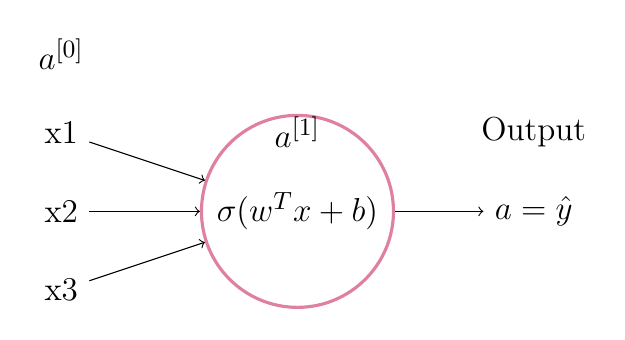
\begin{tikzpicture}
    % Input Layer
    \foreach \name/\i in {x1/1,x2/2,x3/3} {
        \node (Input-\i) at (0,-\i) {\name};
        \ifnum \i=1
            \node[above of=Input-\i] {$a^{[0]}$};
        \fi
    }
    % Hidden Layer
    \foreach \i in {1} {
        \node[circle, minimum size = 6mm, draw=purple!50, line width=.4mm] (Hidden1-\i) at (3,-2) {$\sigma(w^T x + b)$};
        \ifnum \i=1
        \node[above of=Hidden1-\i] {$a^{[1]}$};
        \fi
    }
    % Output Layer
    \foreach \name/\i in {$a=\hat{y}$/1} {
        \node (Output-\i) at (6,-2) {\name};
        \ifnum \i=1
        \node[above of=Output-\i] {Output};
        \fi
    }
    % Arrows
    \foreach \i in {1,2,3} {
        \foreach \j in {1} {
           \draw[->] (Input-\i) -- (Hidden1-\j);
        }
    }
    \foreach \i in {1} {
        \foreach \j in {1} {
            \draw[->] (Hidden1-\i) -- (Output-\j);
        }
    }
\end{tikzpicture}

Each circle(node) represents 2 steps of calculation:\\

$\fbox{$z = w^T x + b$}$\\

$\fbox{$a = \sigma(z)$}$\\

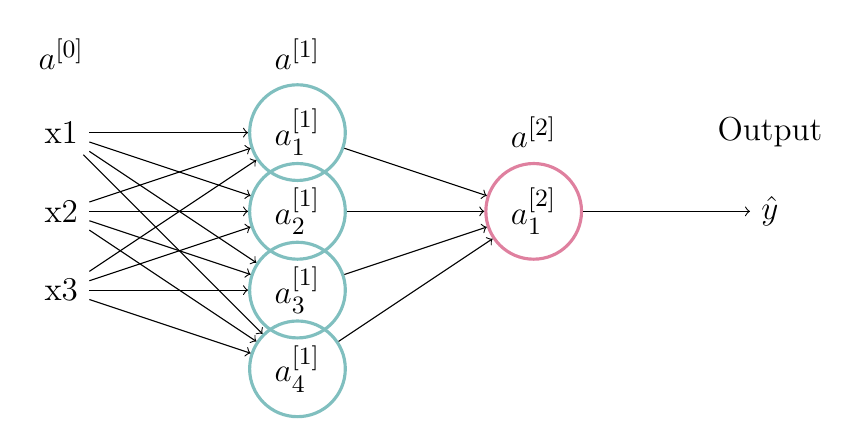
\begin{tikzpicture}
    % Input Layer
    \foreach \name/\i in {x1/1,x2/2,x3/3} {
        \node (Input-\i) at (0,-\i) {\name};
        \ifnum \i=1
            \node[above of=Input-\i] {$a^{[0]}$};
        \fi
    }
    % Hidden Layer
    \foreach \i in {1,2,3,4} {
        \node[circle, minimum size = 6mm, draw=teal!50, line width=.4mm] (Hidden1-\i) at (3,-\i) {$a_{\i}^{[1]}$};
        \ifnum \i=1
        \node[above of=Hidden1-\i] {$a^{[1]}$};
        \fi
    }
    \foreach \i in {1} {
        \node[circle, minimum size = 6mm, draw=purple!50, line width=.4mm] (Hidden2-\i) at (6,-2) {$a_{\i}^{[2]}$};
        \ifnum \i=1
        \node[above of=Hidden2-\i] {$a^{[2]}$};
        \fi
    }
    % Output Layer
    \foreach \name/\i in {$\hat{y}$/1} {
        \node (Output-\i) at (9,-2) {\name};
        \ifnum \i=1
        \node[above of=Output-\i] {Output};
        \fi
    }
    % Arrows
    \foreach \i in {1,2,3} {
        \foreach \j in {1,2,3,4} {
           \draw[->] (Input-\i) -- (Hidden1-\j);
        }
    }
    \foreach \i in {1,2,3,4} {
        \foreach \j in {1} {
           \draw[->] (Hidden1-\i) -- (Hidden2-\j);
        }
    }
    \foreach \i in {1} {
        \foreach \j in {1} {
            \draw[->] (Hidden2-\i) -- (Output-\j);
        }
    }
\end{tikzpicture}

$z_{1}^{[1]} = {w_{1}^{[1]}}^T x + b_{1}^{[1]} \rightarrow a_{1}^{[1]} = \sigma(z_{1}^{[1]})$\\

$z_{2}^{[1]} = {w_{2}^{[1]}}^T x + b_{2}^{[1]} \rightarrow a_{2}^{[1]} = \sigma(z_{2}^{[1]})$\\\\


$a^{[1]} =
\begin{bmatrix}
a_{1}^{[1]} \\
a_{2}^{[1]} \\
a_{3}^{[1]} \\
a_{4}^{[1]} \\
\end{bmatrix}
=
\begin{bmatrix}
\sigma(z_{1}^{[1]}) \\
\sigma(z_{2}^{[1]}) \\
\sigma(z_{3}^{[1]}) \\
\sigma(z_{4}^{[1]}) \\
\end{bmatrix}
=
\begin{bmatrix}
\sigma({w_{1}^{[1]}}^T x +b_{1}^{[1]}) \\
\sigma({w_{2}^{[1]}}^T x +b_{2}^{[1]}) \\
\sigma({w_{3}^{[1]}}^T x +b_{3}^{[1]}) \\
\sigma({w_{4}^{[1]}}^T x +b_{4}^{[1]}) \\
\end{bmatrix}
=
\sigma[
\begin{bmatrix}
\dots & {w_{1}^{[1]}}^T & \dots \\
\dots & {w_{2}^{[1]}}^T & \dots \\
\dots & {w_{3}^{[1]}}^T & \dots \\
\dots & {w_{4}^{[1]}}^T & \dots \\
\end{bmatrix}
\begin{bmatrix}
x_{1} \\
x_{2} \\
x_{3} \\
\end{bmatrix} +
\begin{bmatrix}
b_{1}^{[1]} \\
b_{2}^{[1]} \\
b_{3}^{[1]} \\
b_{4}^{[1]} \\
\end{bmatrix}
]
$\\

\newpage


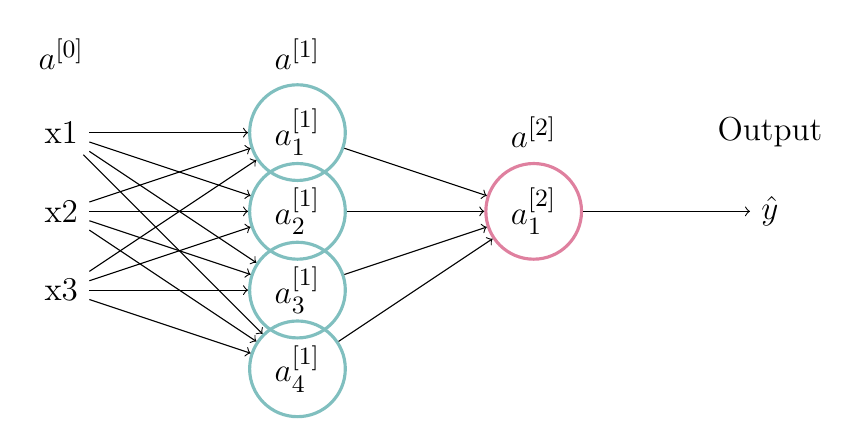
\begin{tikzpicture}
    % Input Layer
    \foreach \name/\i in {x1/1,x2/2,x3/3} {
        \node (Input-\i) at (0,-\i) {\name};
        \ifnum \i=1
            \node[above of=Input-\i] {$a^{[0]}$};
        \fi
    }
    % Hidden Layer
    \foreach \i in {1,2,3,4} {
        \node[circle, minimum size = 6mm, draw=teal!50, line width=.4mm] (Hidden1-\i) at (3,-\i) {$a_{\i}^{[1]}$};
        \ifnum \i=1
        \node[above of=Hidden1-\i] {$a^{[1]}$};
        \fi
    }
    \foreach \i in {1} {
        \node[circle, minimum size = 6mm, draw=purple!50, line width=.4mm] (Hidden2-\i) at (6,-2) {$a_{\i}^{[2]}$};
        \ifnum \i=1
        \node[above of=Hidden2-\i] {$a^{[2]}$};
        \fi
    }
    % Output Layer
    \foreach \name/\i in {$\hat{y}$/1} {
        \node (Output-\i) at (9,-2) {\name};
        \ifnum \i=1
        \node[above of=Output-\i] {Output};
        \fi
    }
    % Arrows
    \foreach \i in {1,2,3} {
        \foreach \j in {1,2,3,4} {
           \draw[->] (Input-\i) -- (Hidden1-\j);
        }
    }
    \foreach \i in {1,2,3,4} {
        \foreach \j in {1} {
           \draw[->] (Hidden1-\i) -- (Hidden2-\j);
        }
    }
    \foreach \i in {1} {
        \foreach \j in {1} {
            \draw[->] (Hidden2-\i) -- (Output-\j);
        }
    }
\end{tikzpicture}

Given input $x$:\\

$z^{[1]} = W^{[1]} a^{[0]} + b^{[1]}$, where $_{(4,1) = (4,3)(3,1)+ (4,1)}$\\

$a^{[1]} = \sigma(z^{[1]})$\\

$z^{[2]} = W^{[2]}a^{[1]} + b^{[2]}$, where $_{(1,1) = (1,4)(4,1)+ (1,1)}$\\

$a^{[2]} = \sigma(z^{[2]})$\\

\newpage
\subsection{Vectorizing Across Multiple Examples}

for $i=1$  to $m$:\\

$z^{[1](i)} = W^{[1]} x^{(i)} + b^{[1]}$\\

$a^{[1](i)} = \sigma(z^{[1](i)})$\\

$z^{[2](i)} = W^{[2]}a^{[1](i)} + b^{[2]}$\\

$a^{[2](i)} = \sigma(z^{[2](i)})$\\


\newpage
\subsection{}

\end{document}

